\documentclass{standalone}
\usepackage{tikz}

\usetikzlibrary{calc,math}


\begin{document}

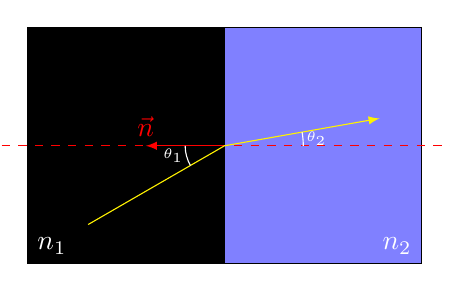
\begin{tikzpicture}
  \path[use as bounding box] (0,0) rectangle (5,3);
  \draw[fill=black] (0,0) rectangle (5,3);
  \draw[fill=blue!50] (2.5,0) rectangle (5,3);

  \coordinate (P) at (2.5,1.5);

  \draw[red,-latex] (P) -- ++(-1,0) node[above] {$\vec n$};
  \draw[red,dashed,thin] ($ (P) + (-10,0) $) -- ++(20,0);

  \node[anchor=south west,white] at (0,0) {$n_1$};
  \node[anchor=south east,white] at (5,0) {$n_2$};

  \draw[yellow,-latex] ($ (P) + (30:-2) $) -- (P) -- ++(10:2);

  \draw[white] ($ (P) + (180:0.5) $) arc [radius=0.5,start angle=180,delta angle=30] node[midway,left,font=\tiny,inner sep=1pt] {$\theta_1$};
  \draw[white] ($ (P) + (0:1) $) arc [radius=1,start angle=0,delta angle=10] node[midway,right,font=\tiny,inner sep=1pt] {$\theta_2$};
\end{tikzpicture}

\end{document}